\documentclass[12pt,french]{article} %ajouter draft pour voir débordement
\usepackage[utf8]{inputenc}
\usepackage[T1]{fontenc}
\usepackage{lmodern}
%règles mes marges et format papier
\usepackage[a4paper,hmargin=2cm,vmargin=2cm]{geometry} %modif marge et formet
\usepackage{amsmath, amssymb, amsthm}
\usepackage{fancyhdr} %pour les entêtes et bas de page
\usepackage{lastpage} %pour numéroter les pages charge la derniere page
\usepackage{graphicx} %pour inclure des img
\usepackage{dsfont}
\usepackage{float} %pour le placement des figures
\usepackage{hyperref} %pour mettre des liens hypertext
\usepackage{calc} %permet de calculer les marges pour encadrer les textes
\usepackage{color, xcolor} %gère les couleurs
\usepackage{babel}
\usepackage{listings} %pour afficher le code annexe

%pour afficher le code de manière esthétique
\lstset{
  aboveskip=3mm,
  belowskip=-2mm,
  backgroundcolor=\color{white},
  basicstyle=\footnotesize,
  breakatwhitespace=false,
  breaklines=true,
  captionpos=b,
  commentstyle=\color{red},
  deletekeywords={...},
  escapeinside={\%*}{*)},
  extendedchars=true,
  framexleftmargin=16pt,
  framextopmargin=3pt,
  framexbottommargin=6pt,
  frame=tb,
  keepspaces=true,
  keywordstyle=\color{blue},
  language=C,
  literate=
  {²}{{\textsuperscript{2}}}1 {⁴}{{\textsuperscript{4}}}1
  {⁶}{{\textsuperscript{6}}}1
  {⁸}{{\textsuperscript{8}}}1
  {€}{{\euro{}}}1 {é}{{\'e}}1 {è}{{\`{e}}}1 {ê}{{\^{e}}}1 {ë}{{\¨{e}}}1
  {É}{{\'{E}}}1 {Ê}{{\^{E}}}1 {û}{{\^{u}}}1 {ù}{{\`{u}}}1 {â}{{\^{a}}}1
  {à}{{\`{a}}}1 {á}{{\'{a}}}1 {ã}{{\~{a}}}1 {Á}{{\'{A}}}1 {Â}{{\^{A}}}1
  {Ã}{{\~{A}}}1 {ç}{{\c{c}}}1 {Ç}{{\c{C}}}1 {õ}{{\~{o}}}1 {ó}{{\'{o}}}1 
  {ô}{{\^{o}}}1 {Õ}{{\~{O}}}1 {Ó}{{\'{O}}}1 {Ô}{{\^{O}}}1 {î}{{\^{i}}}1
  {Î}{{\^{I}}}1 {í}{{\'{i}}}1 {Í}{{\~{Í}}}1,
  morekeywords={*,...},
  numbers=left,
  numbersep=10pt,
  numberstyle=\tiny\color{black},
  rulecolor=\color{black},
  showspaces=false,
  showstringspaces=false,
  showtabs=false,
  stepnumber=1,
  stringstyle=\color{gray},
  tabsize=4,
}
%%%%%

%Personalisation En tête
\pagestyle{fancy}
\renewcommand\headrulewidth{1pt}
%permet d'aumenter tailler header pour mettre image (31pt ici)
\setlength{\headheight}{31pt} 
\fancyhead[L]{Architecture Logiciel \\ et Qualité}
\fancyhead[C]{
\includegraphics[scale=0.28]{header.png}}
\fancyhead[R]{Dossier Analyse \\ Métier}
\renewcommand\footrulewidth{1pt}
\fancyfoot[L]{SMAirport}
\fancyfoot[C]{\thepage/\pageref{LastPage}}
\fancyfoot[R]{2022/2023}
%Fin personalisation En Tête


\begin{document}

\begin{titlepage} %page d'acceuil

  
  
\includegraphics[scale=0.6]{isima.png}
  \hspace*{\stretch{1}}%espace horizontal entre les 2 images
  
\includegraphics[scale=0.2]{deco.jpg}
  
  \vspace*{2.5cm} %espace de 2.5cm en dessous des images
  
  \begin{center}\huge
    \textbf{Dossier Analyse Métier} 
    
    \textbf{SMAirport}
  \end{center}
  
  \hrule %trait horizontal
  
  \begin{center}
    \Large BALLEJOS Lilian,
    \Large CHARPIN Etienne et
    \Large DENIZOT Hugo
    
    \large
    
    ISIMA INP
  
    Année Universitaire 2022/2023
  \end{center}
  
  \begin{center}
    %créer une boite ou mettre l'image qui fait la largeur de la page
    \makebox[\textwidth]{
\includegraphics[width=\paperwidth]{garde.png}}
  \end{center}
  
  \vspace*{2cm} 
  
  \begin{flushright}\footnotesize %a droite
    Enseignant référant: Mr HILL David
    
    Date du rendu: 16 janvier 2023
    
  \end{flushright}
  
  \begin{flushleft}\small %a gauche
    \textbf{ISIMA}
    \footnotesize
    
    1 rue de la Chebarde - TSA 60125 - CS 60026 - 63178 Aubière CEDEX
    
    Tel: 04 73 40 50 00
    
    Site web: \href{https://www.isima.fr/}{isima.fr}\newline
    	
  \end{flushleft}
\end{titlepage}	


%Ma table des Matières !
%permet de renommer 'table des matières' en sommaire
\renewcommand{\contentsname}{Sommaire}
\normalsize\tableofcontents %place la table des matières

\bigskip

\section{Introduction}

Nous allons vous présenter aujourd'hui dans ce dossier les prémices de notre futur programme de \textbf{SMA} (simulation multi-agents).

\bigskip

Il s'agit d'une simulation qui sera composé de douanier et de client lambda qui interagiront les uns avec les autres dans un aéroport.

\bigskip

 Nous nous concentrerons sur les différents checks que les clients doivent passer, notamment les files d'attente, les fouilles de sécurité et la récupération des bagages. Nous allons également prendre en compte les actions possibles pour les différents agents, comme les douaniers qui peuvent fouiller les clients et les arrêter s'ils ne sont pas en règle. L'objectif de ce projet est d'analyser les différents processus et les interactions entre les agents pour comprendre comment ils contribuent au bon fonctionnement de l'aéroport
 
 \bigskip
 
 \textbf{Remarque:}
 

Notre projet sera disponible sur le Gitlab de l'ISIMA INP en protection \textit{internal} ce qui signifie que pour y accéder il faut être connecté à celui-ci.

Retrouver notre projet en suivant ce lien: \href{https://gitlab.isima.fr/liballejos/smairport}{ici}

\newpage

\section{Choix du langage}

Nous avons décidé de coder ce programme en \textbf{C++} pour deux raisons:

\medskip

\begin{itemize}
	\item Ce langage est performant car plus proche de la machine et sera donc plus efficace et plus rapide pour effectuer une SMA (des programmes qui sont parfois très lourd)
	
	\item Cela nous permettra de nous améliorer dans ce langage que nous étudions en ce moment en cours et sur lequel nous serons évalués.
\end{itemize}



\section{Objectifs}

Nous sommes dans la zone d'entrée d'un aéroport.

L'agent "Client" se déplace entre les différentes parties de l'aéroport et interagit avec celles-ci .

L'agent douanier lui interagit avec les clients en les fouillant et les arrêtes si ceux-ci ne sont pas en règle.

\section{Conception du programme}

\subsection{Théorie}

Il nous faut deux agents:

\begin{itemize}
	\item Le visiteur: représente le client, il se déplace dans les différentes parties de l'aéroport et interagi avec
	
	\item Le douanier: ll se déplace aussi entre les différentes parties de l'aéroport mais lui va arrêter les clients pour les contrôler
\end{itemize}

\subsection{Diagramme de cas d'utilisation}

Voici un diagramme de cas d'utilisation qui représente notre futur simulation.

\begin{figure}[H]
	\centering
	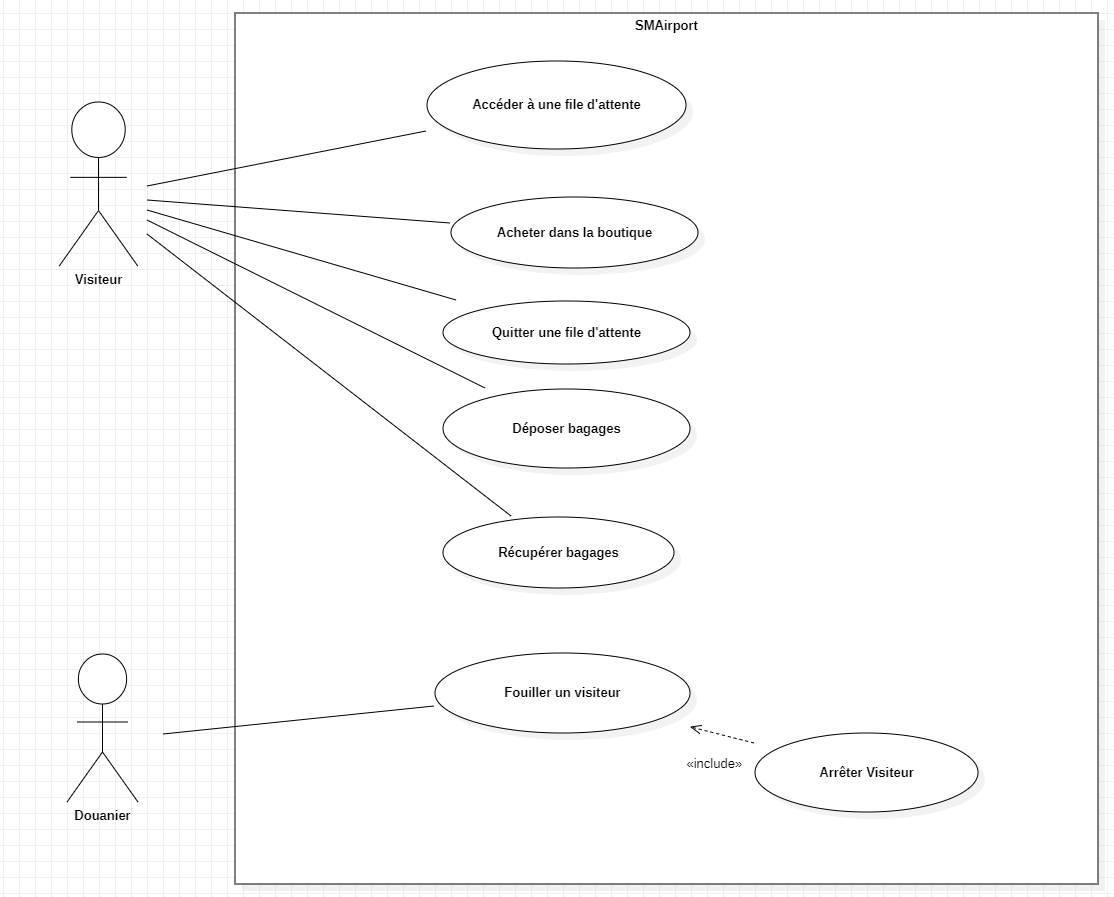
\includegraphics[scale=0.285]{usecase.png}
	\caption{Diagramme de cas d'utilisation}    
\end{figure}

\section{Analyse du programme}

\subsection{Analyse}

Nos deux types d'agents seront tous des personnes.

L'aéroport est composé de différents éléments qui le \textbf{compose} comme la zone d'embarquement, la boutique et la zone de bagages

Les visiteurs interagissement entre eux et avec les différents éléments de l'aéroport.

Les douaniers interagissent avec les visiteurs. 


\subsection{Diagramme de classe d'analyse}

\subsubsection{Le diagramme}

Voici un diagramme de classe d'analyse qui réparti et défini les différents éléments de notre future simulation.

\begin{figure}[H]
	\centering
	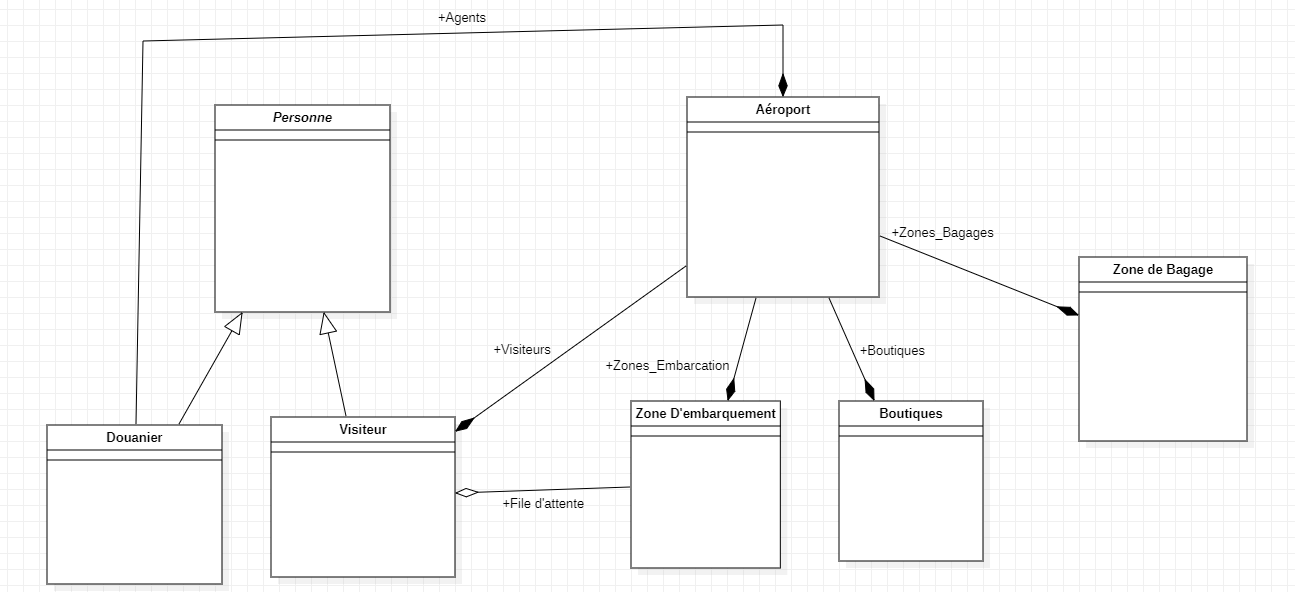
\includegraphics[scale=0.4]{analyse.png}
	\caption{Diagramme de classe d'analyse}    
\end{figure}

\subsubsection{Explication des choix}

Nous avons mis des compositions pour les différents éléments de l'aéroport (Boutiques par exemple) car sans aéroport ces éléments sont voués à disparaitre car inutile.

Nous avons considéré cependant que les visiteurs et douaniers sont par contre des agrégations car pas forcément rattachés à un aéroport précis. Si l'aéroport viendrait à disparaitre, il ne faudrait pas forcément supprimer les agents.

Nous avons de plus, choisis de faire une agrégation par type d'agent car ils n'ont pas le même rôle dans l'aéroport. Nous n'avons donc pas mit une agrégation générale sur "\textit{Personne}". 


\section{Planification des tâches}

Nous nous sommes répartis temporellement les différentes tâches à faire et l'avons représenté visuellement à l'aide d'un Gantt.

\begin{figure}[H]
	\centering
	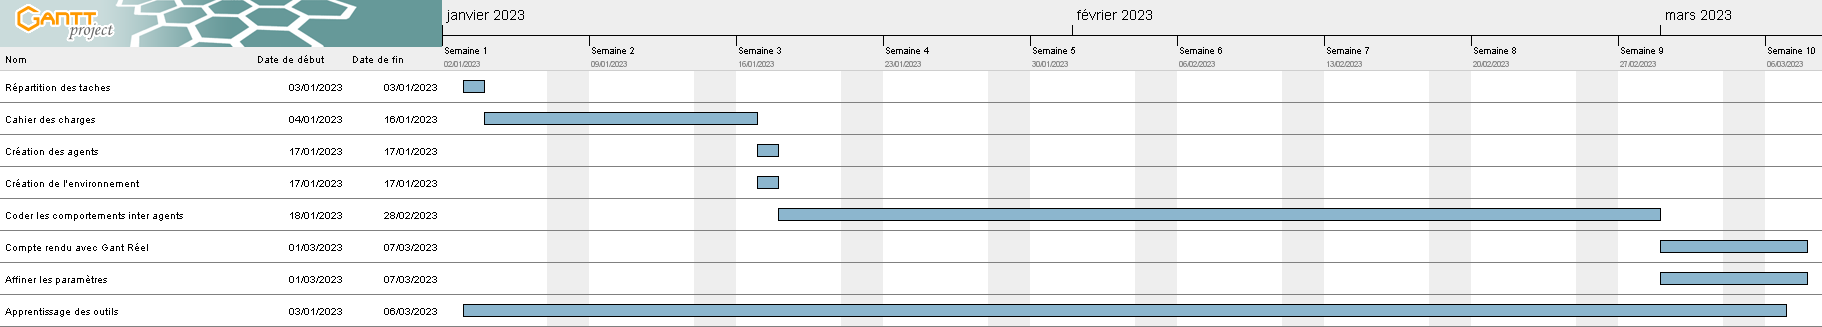
\includegraphics[scale=0.35]{gantt.png}
	\caption{Gantt prévisionnel}    
\end{figure}

\bigskip

Ce Gantt vous sera aussi fourni à côté du rapport car il n'est pas parfaitement lisible incrusté ici dans le pdf.

\section{Les spécialisations pour chaque membre du binôme}

Nous avons tous choisis une spécialité à approfondir durant ce sujet de TP afin de nous améliorer dans un domaine.

\subsection{Choix de BALLEJOS Lilian}

Lilian se spécialisera dans l'intégration continue avec l'outil GitlabCI.

\begin{figure}[H]
	\centering
	
\includegraphics[scale=0.35]{clilian.png}
	\caption{GitlabCI}    
\end{figure}



\subsection{Choix de CHARPIN Etienne}

Etienne se spécialisera dans l'étude des performances à l'aide de l'outil SonarQube.

\begin{figure}[H]
	\centering
	
\includegraphics[scale=0.35]{cetienne.png}
	\caption{SonarQube}    
\end{figure}


\subsection{Choix de DENIZOT Hugo}

Hugo se spécialisera dans la production de documentation à l'aide de l'outil Doxygen.

\begin{figure}[H]
	\centering
	
\includegraphics[scale=0.35]{chugo.png}
	\caption{Doxygen}    
\end{figure}


\bigskip


\listoffigures


\end{document}
